\chapter{Background}~\label{chp:Background}

This chapter covers the different topics that are present in this thesis and is structured as followed:
\begin{itemize}
\item Sections~\ref{sec:cmp} and \ref{sec:hcmp} cover Chip Multicore Processors and Heterogeneous Chip Multicore Processors to motivate the use of Dynamic Multicore Processors (DMP).
\item Section~\ref{sec:dmp}  describes the three types of DMP that currently exists.
\item Section~\ref{chp:bg:sec:edge} describes the Explicit Data Graph Execution (EDGE) instruction set architecture (ISA) used by the DMP explored throughout this thesis.
Subsection~\ref{sec:edge_isa} explains how EDGE blocks are formed, which is useful for Chapter~\ref{chp:streamit} and Chapter~\ref{chp:cases}.
Subsection~\ref{sec:edge_arch} covers how blocks are executed on a single core, as well how they are executed when the processor is reconfigured, this is important knowledge for Chapters~\ref{chp:streamit}, \ref{chp:cases} and \ref{chp:hardchanges}.
\item Section~\ref{sec:valpred} explains how value predictors works, this is used in Chapter~\ref{chp:hardchanges}.
\item Section~\ref{sec:bg:stream} describes streaming programming languages, explored in Chapter~\ref{chp:streamit}.
\item Section~\ref{sec:ml} covers the different machine learning techniques and evaluation methods used.
Linear regression, described in subsection~\ref{sec:lr} is used in both Chapter~\ref{chp:streamit} and \ref{chp:cases}.
k Nearest Neighbors explained in subsection~\ref{sec:kNN} is used in Chapter~\ref{chp:streamit}, k-means clustering found at subsection~\ref{sec:kMeans} is used in Chapter~\ref{chp:cases}.
Leave-one cross validation described in subsection~\ref{sec:valid} is used in Chapter~\ref{chp:streamit} and \ref{chp:cases}.
\item Finally, Section~\ref{sec:esc} explains the Early Stopping Criterion used in Chapter~\ref{chp:streamit}.
\end{itemize}
%Sections~\ref{sec:cmp} and \ref{sec:hcmp} cover Chip Multicore Processors and Heterogeneous Chip Multicore Processors to motivate the existence and research conducted in Dynamic Multicore Processors (DMP).
%This is followed by Section~\ref{sec:dmp} that describes of the three types of Dynamic Multicore Processors that currently exists.
%Then the Explicit Data Graph Execution (EDGE) instruction set architecture (ISA) is described in section~\ref{sec:edge_isa}; this is the ISA used by the DMP explored throughout this thesis.
%Specific features of an EDGE Processor, including the ability to fuse cores is then explained in detail (section~\ref{sec:edge_arch}).
%Value prediction, and more specifically the differential value TAGE (D-VTAGE) value predictor is described in section~\ref{
%Finally, streaming programming languages, which are used in Chapter~ref{}, and the different machine learning techniques utilised in the thesis are explained.

\section{Chip Multicore Processors}~\label{sec:cmp}

\begin{figure}[t]
 \center
 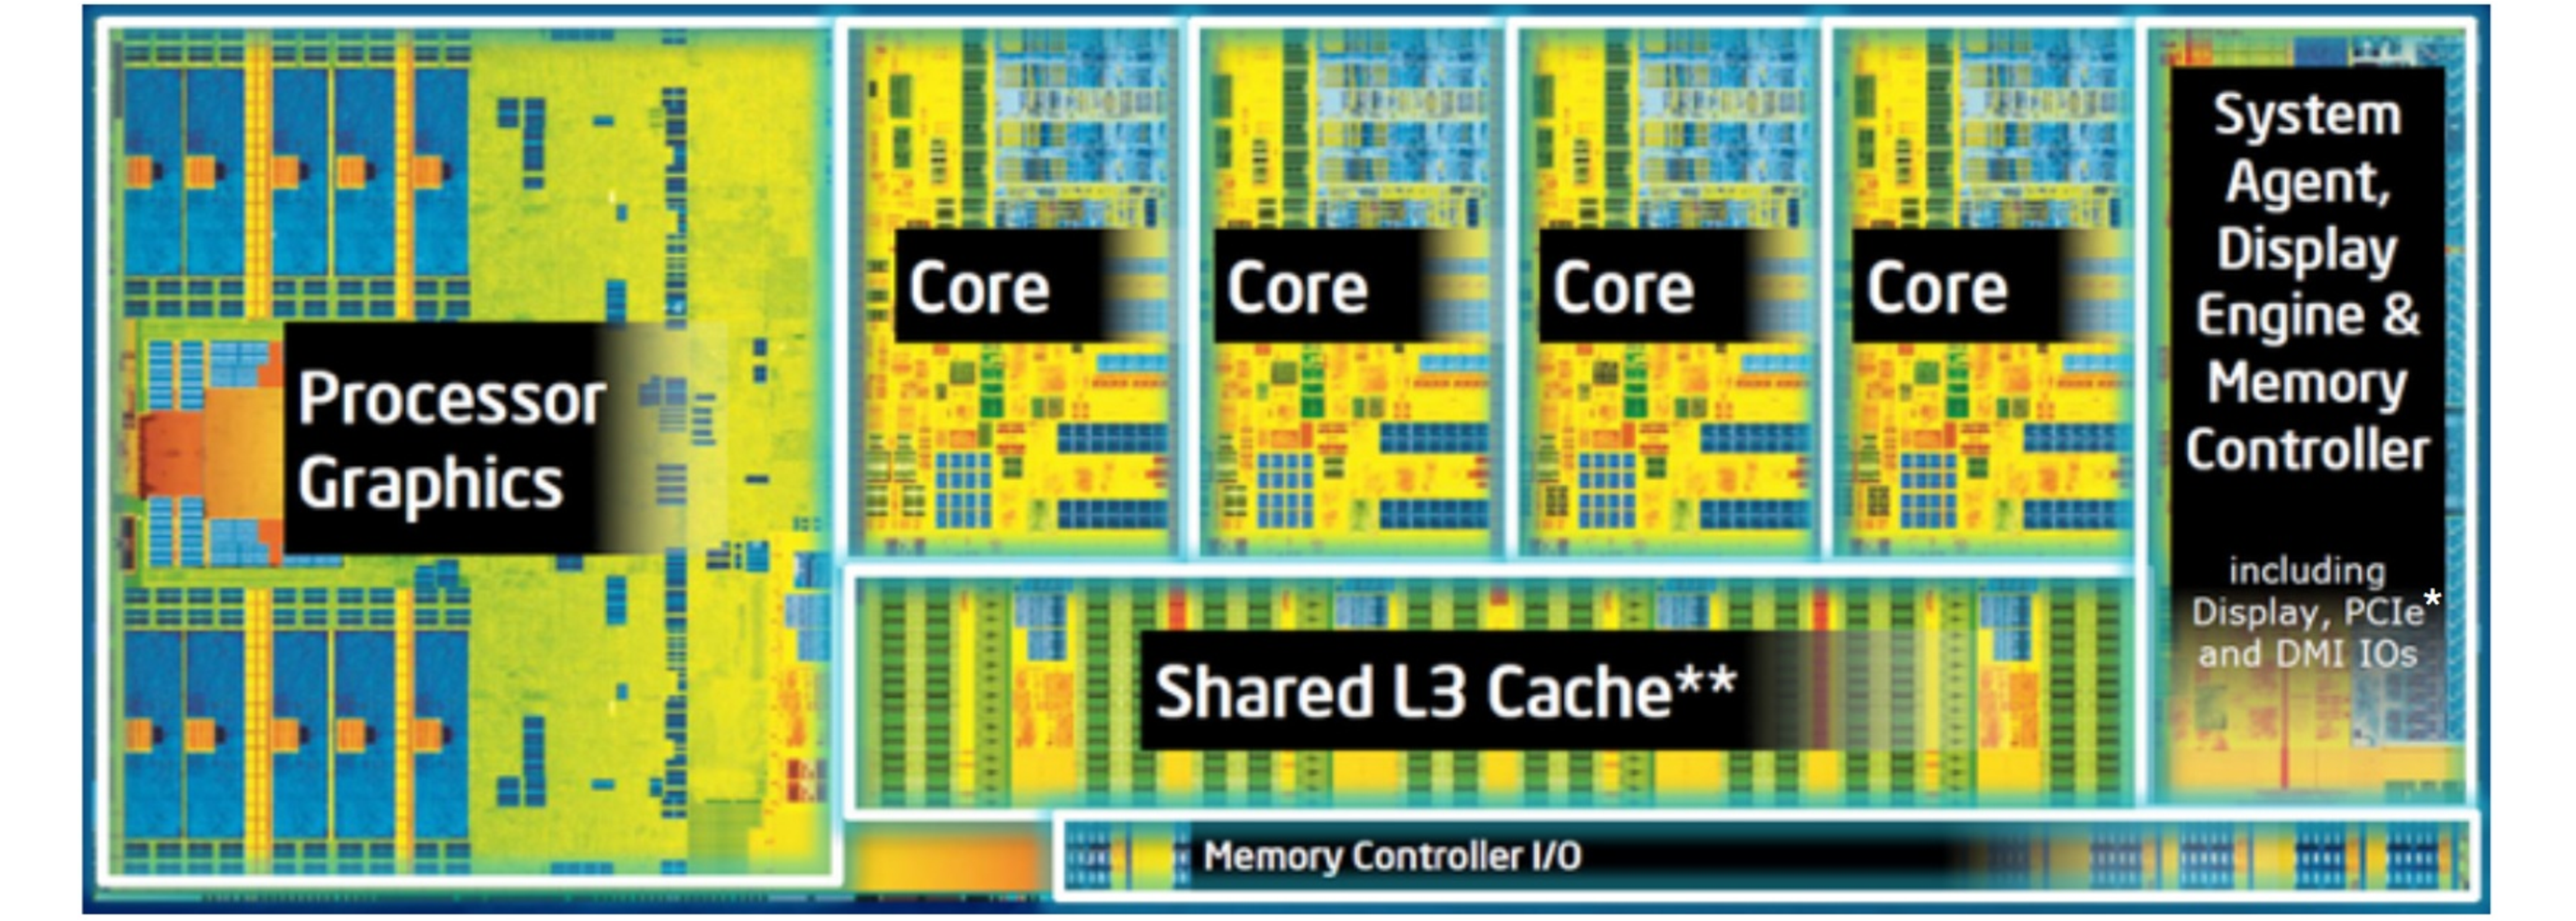
\includegraphics[width=1\textwidth]{background/graphics/i7intel.pdf}
 \caption{Intel Core i7 processor internal die photograph taken from~\cite{turleywhite}}\label{fig:i7}
\end{figure}
 
Chip Multicore Processors (CMPs) are now ubiquitous due to the difficulty in scaling single core performance.
In a CMP, multiple processor cores are packaged on a single die as seen in Figure~\ref{fig:i7}.
The most commonly adopted CMP design features homogeneous cores as it reduces the design complexity from a hardware perspective~\cite{asanovic2006landscape}.
In a CMP the performance improvement come from running multiple tasks in parallel.
These tasks can either be different programs or multiple threads from a single program executing on multiple cores.

The performance benefits of executing a program on a CMP can be estimated using Amdahl's Law~\cite{amdahl1967validity}.
It states that the speedup \textit{S} obtained by executing a program on \textit{n} cores depends on the fraction of work which is parallelisable \textit{f}.

\begin{equation}
S = \frac{1}{(1-f) + \frac{f}{n}}
\end{equation}\label{amdlaw}

If a CMP features an infinite number of cores~\cite{eyerman2010amdahl}, then Amdahl's law can be rewritten as:

\begin{equation}
\lim_{n\to\infty} S = \frac{1}{(1-f)}
\end{equation}

Therefore, given any program, the speedup obtained through using a CMP is limited to the fraction \textit{f} of parallel work found in the program.
As all the cores are homogeneous, if the parallel fraction is low, then this causes serial bottlenecks to reduce the potential speedup, as no core will be specialised for single-threaded execution.
%This implication has pushed research into finding ways of parallelising code to its fullest~\cite{}, however this may not always be possible~\cite{}.
%Thus whilst CMPs have become a mainstain in processor design, the homogeneous model has its limits.
\section{Heterogeneous Chip Multicore Processors}~\label{sec:hcmp}

\begin{figure}[t]
 \center
 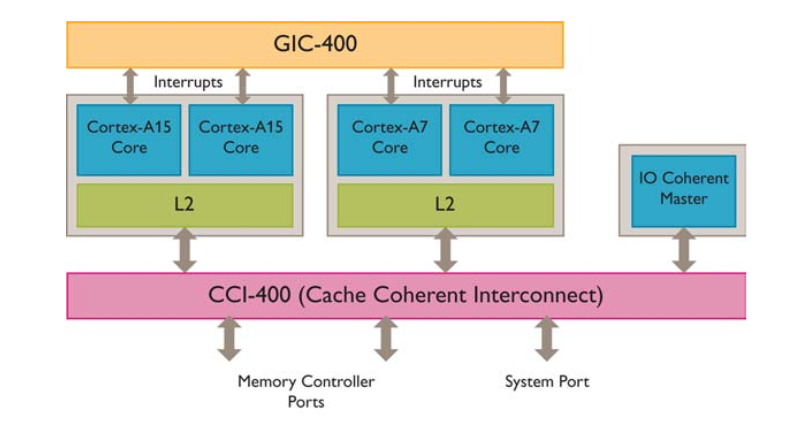
\includegraphics[width=1\textwidth]{background/graphics/biglittle.png}
 \caption{Example of a heterogeneous multicore processor proposed by ARM (big.LITTLE)~\cite{armbig}}\label{fig:blarm}
\end{figure}
\vspace{-1em}

Unlike CMPs, Heterogeneous Chip Multicore Processors (HCMPs) bring a variety of cores onto a single package.
This variety may come in different forms, such as having multiple instruction set architectures (ISA) on the same system on chip (MPSoCs)~\cite{venkat2014harnessingisa,venkatHipstr2016}, different size cores on an SoC~\cite{armbig,jeff2012big}.
Figure~\ref{fig:blarm} shows a schemata for ARM's big.LITTLE HCMP, where a high-performance Cortex-A15 is paired with a simpler, power efficient Cortex-A7.
The two cores are connected via a cache coherent interconnect which provides data coherence at the bus-level, allowing the cores to make reads to its neighbor~\cite{armbig}.
Software is then executed on one of the cores depending on the user's requirement.

This example demonstrates an advantage of HCMPs; unlike CMPs, the variety of cores provide a flexibility to the hardware.
This can be used for different purposes, such as security~\cite{venkatHipstr2016}, energy/power savings~\cite{venkat2014harnessingisa} and speeding up applications~\cite{venkat2014harnessingisa}.
In their 2014 paper, Venkat et al.~\cite{venkat2014harnessingisa} demonstrate that a multi-ISA HCMP can improve performance by up to 1.4x and achieve energy savings of up to 40\% compared to a CMP on a peak-power budget of 40W.
They motivate the idea that HCMPs with heterogeneous ISAs even improve over the performance of single-ISA HCMPs with speedups around 15\% and energy savings of 21.5\%.

\begin{figure}[t]
    \centering
    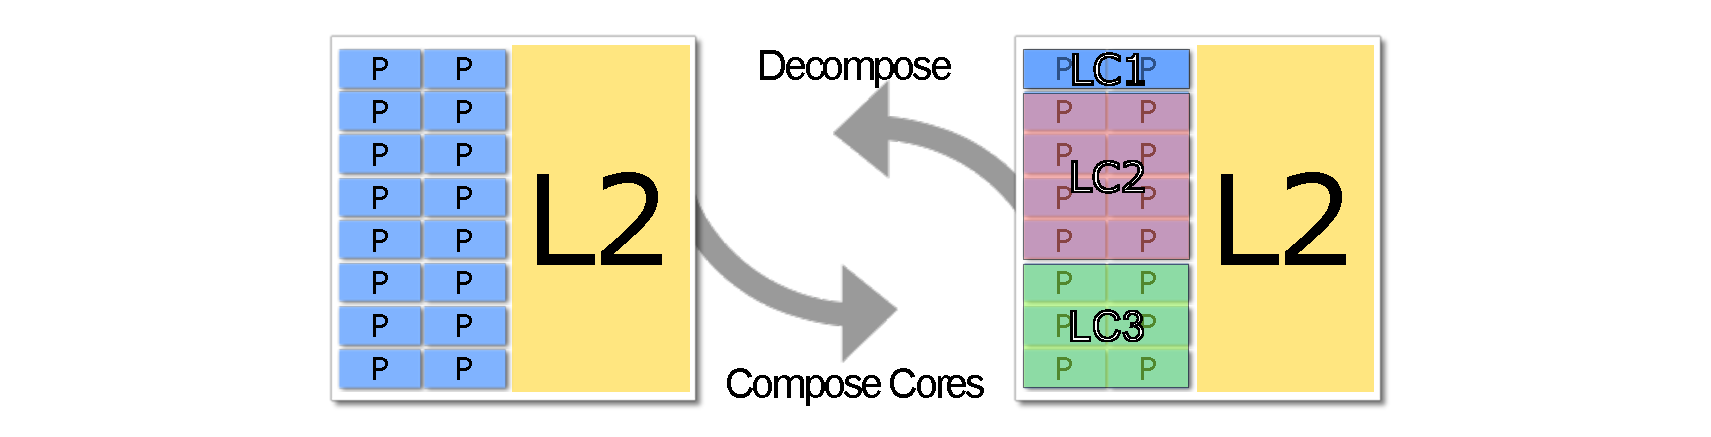
\includegraphics[width=1\textwidth]{background/graphics/cmp_new.pdf}
    \caption{High-level view of a DMP that can modify its core count.}
    \label{fig:dynmulticore}
	\vspace{-0.5em}
\end{figure}
Whilst the hardware diversity in HCMPs is an advantage compared to CMPs, it increases the complexity of the optimisation space.
For example, Gupta et al. in ~\cite{Gupta2017Dypo} show that a single-ISA octa-core big.LITTLE architecture can have 20 different CPU core configurations, combined with the ability to dynamically modify the voltage, this leads to 4000 unique possible hardware configurations to choose from at runtime.
This highly increases the complexity of obtaining the correct settings for different programs.
MPSoCs also face a similar issue as having more than a single ISA not only adds design challenges, but program migration between different cores may in fact deteriorate performance~\cite{DeVuystMigration2012}.
\vspace{-1em}
\section{Dynamic Multicore Processors}~\label{sec:dmp}
\vspace{-1em}

In both CMPs and HCMPs, the design of the processor is fixed, meaning that many of the trade-offs between power, performance and area cannot be changed after production.
Dynamic Multicore Processors (DMPs) attempt to bridge the gap between the two previous designs by allowing the execution substrate to adapt dynamically at runtime.
Mitall's survey ~\cite{MittalSurv2016} defines three types of modifiable resources: the core count~\cite{ipek2007CoreFusion,kim2007tflex,pricopi2012bahurupi}, number of resources that each core has~\cite{Homayoun3DPooling2012} and microarchitectural features~\cite{fallinhetblock2014,BauerRSE08,tavanaElastic}.

\paragraph*{Core Composition Dynamic Multicore Processors}


A DMP that can modify its core count is composed of homogeneous cores with a reconfigurable fabric.
Physical cores can function either on their own or as a group.
Figure~\ref{fig:dynmulticore} provides an high level view of a DMP: the physical cores \textit{P}, are composed into 3 separate compositions of sizes 2, 8 and 4.
Each of the compositions executes a single thread, leveraging the power of the cores that are grouped together.
A composition fetches instructions from a single source and executes them across all the physical cores that compose it.
Cores can fuse dynamically and create core compositions of any sizes.
The exact mechanism of core composition is described later on in Section~\ref{chp:bg:sec:edge}.

The advantage of a core composition DMP over the traditional CMP or HCMP is the ability to reconfigure the processor dynamically to better match the tasks at hand.
For example, large sequential sections of code with high Instruction Level Parallelism (ILP) can be accelerated on a core composition that mimics a wide superscalar processor.
On parallel workloads the DMP can be reconfigured by de-composing the composition as seen in Figure~\ref{fig:dynmulticore} to match the Thread Level Parallelism (TLP).

\paragraph*{Resource Sharing Dynamic Multicore Processors}
A more fine-grained DMP technique is resource-sharing.
For example in the WiDGET DMP by Watanabe et al. \cite{Watanabe2010Widget}, cores are built out of Instruction Engine front-ends which function similarly to Out of Order (OoO) cores' front and back end pipeline functions.
They then are connected to Execution Units which they can choose to use.
Each core in the WiDGET DMP also have access to their neighbors Execution Units, allowing for more variation.
Another example of resource sharing can be found in Rodrigues et al.'s work~\cite{rodrigues2014perf} where a core can use resources such as Arithmetic Logic Units (ALUs) from other cores.

\paragraph*{Microarchitectural Reconfigurable Dynamic Multicore Processors}
A final example is a DMP which can reconfigure microarchitectural features to better fit the current application.
Fallin et al.~\cite{fallinhetblock2014} observe that serial code can exhibit phases that fit different microarchitectural features.
According to them, these phases may only been in the ten to hundred thousands instructions long.
These DMPs can therefore modify microarchitecural features, such as in-order or out-of-order execution, to best match the current phase of a program.

\section{EDGE}\label{chp:bg:sec:edge}

\begin{figure}[t]
    \centering
    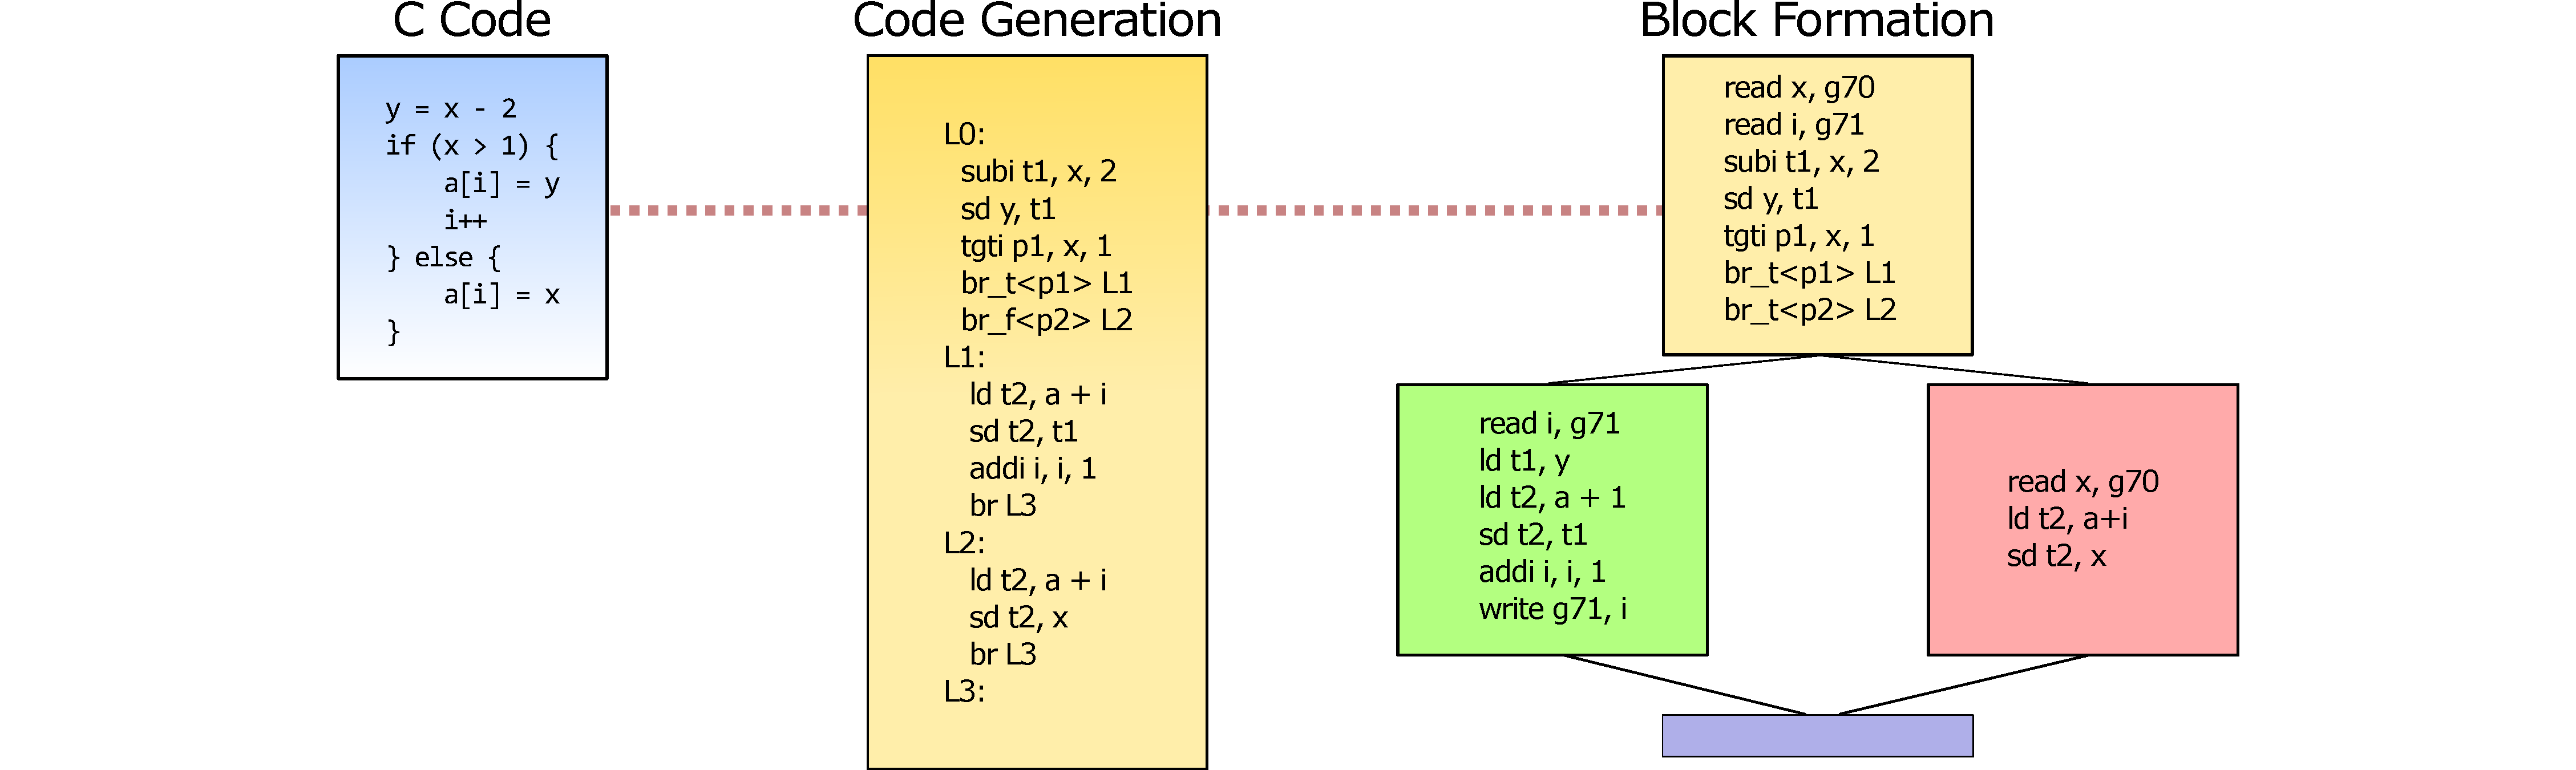
\includegraphics[width=1\textwidth]{background/graphics/EDGE_4.pdf}
    \caption{High-level view of the two main EDGE compiler passes. First pass involves standard optimisations, and code generation. Second pass transforms the code into atomic blocks of instructions.}
    \label{fig:EdgeHigh}
\end{figure}
This section describes the Explicit Data Graph (EDGE) architecture.
First the ISA is covered, with an example of how source code is transformed into blocks of instructions.
Then the features of an EDGE processor are described, such as the ability of executing multiple blocks on a core and how core composition works with EDGE.

\subsection{EDGE Instruction Set Architecture}~\label{sec:edge_isa}

The Explicit Data Graph Execution (EDGE) architecture~\cite{burger04edge} is a dataflow architecture aimed at improving concurrency whilst being energy and power efficient \cite{smith2006edge,burger04edge}.
Similar to very long instruction word (VLIW) architectures that pack multiple sub-instructions into a single instruction, EDGE requires that the compiler structure instructions as blocks.
Unlike VLIW that uses static placement and static issue which puts high pressure on the compiler, EDGE allows for dynamic issue which distributes responsibility between the hardware and the compiler more evenly.

\paragraph*{Block Formation}
In EDGE, instructions are organised into blocks, which are fetched as single units by the processor.
Figure~\ref{fig:EdgeHigh} shows a high-level overview of how EDGE creates the blocks of instructions.
The first pass (Code Generation) transforms source code into a control flow graph (CFG), performing optimisations such as loop unrolling and inlining.
Then, each node of the CFG is turned into an EDGE block given a set of restrictions.
These restrictions are:
\begin{itemize}
\item Block Size: an EDGE block may be between 4 to 128 instructions.
\vspace{-1em}
\item Load/Store: an EDGE block may have at most 32 load/store instructions.
\vspace{-1em}
\item Entry/Exit: an EDGE block may have a single exit but may have multiple exits.
\end{itemize}
If a block does not meet these requirements, it is broken down into smaller blocks.

Unlike traditional ISAs such as x86 or ARM's ISAs, instructions in a block do not communicate via registers, but rather the output targets of instructions are encoded to instruction inputs~\cite{smith2006edge}.
Loads and stores in each EDGE block are assigned unique identifiers which are used resolve load-store dependencies.
Thus, the EDGE architecture encode dependencies between instructions at the ISA level.
Registers are only used for inter-communication between blocks.

An EDGE block also contains a header that will inform the hardware about the number of stores and register writes contained in the block~\cite{smith2006edge}.
This information is used to detect data-dependencies between blocks if multiple blocks are executed in parallel.
For example, if two blocks write to the same register, then the register-file can detect which one must fire the write first based on the header information. 

\paragraph*{Hyperblock formation}
\begin{figure}[t]
    \centering
    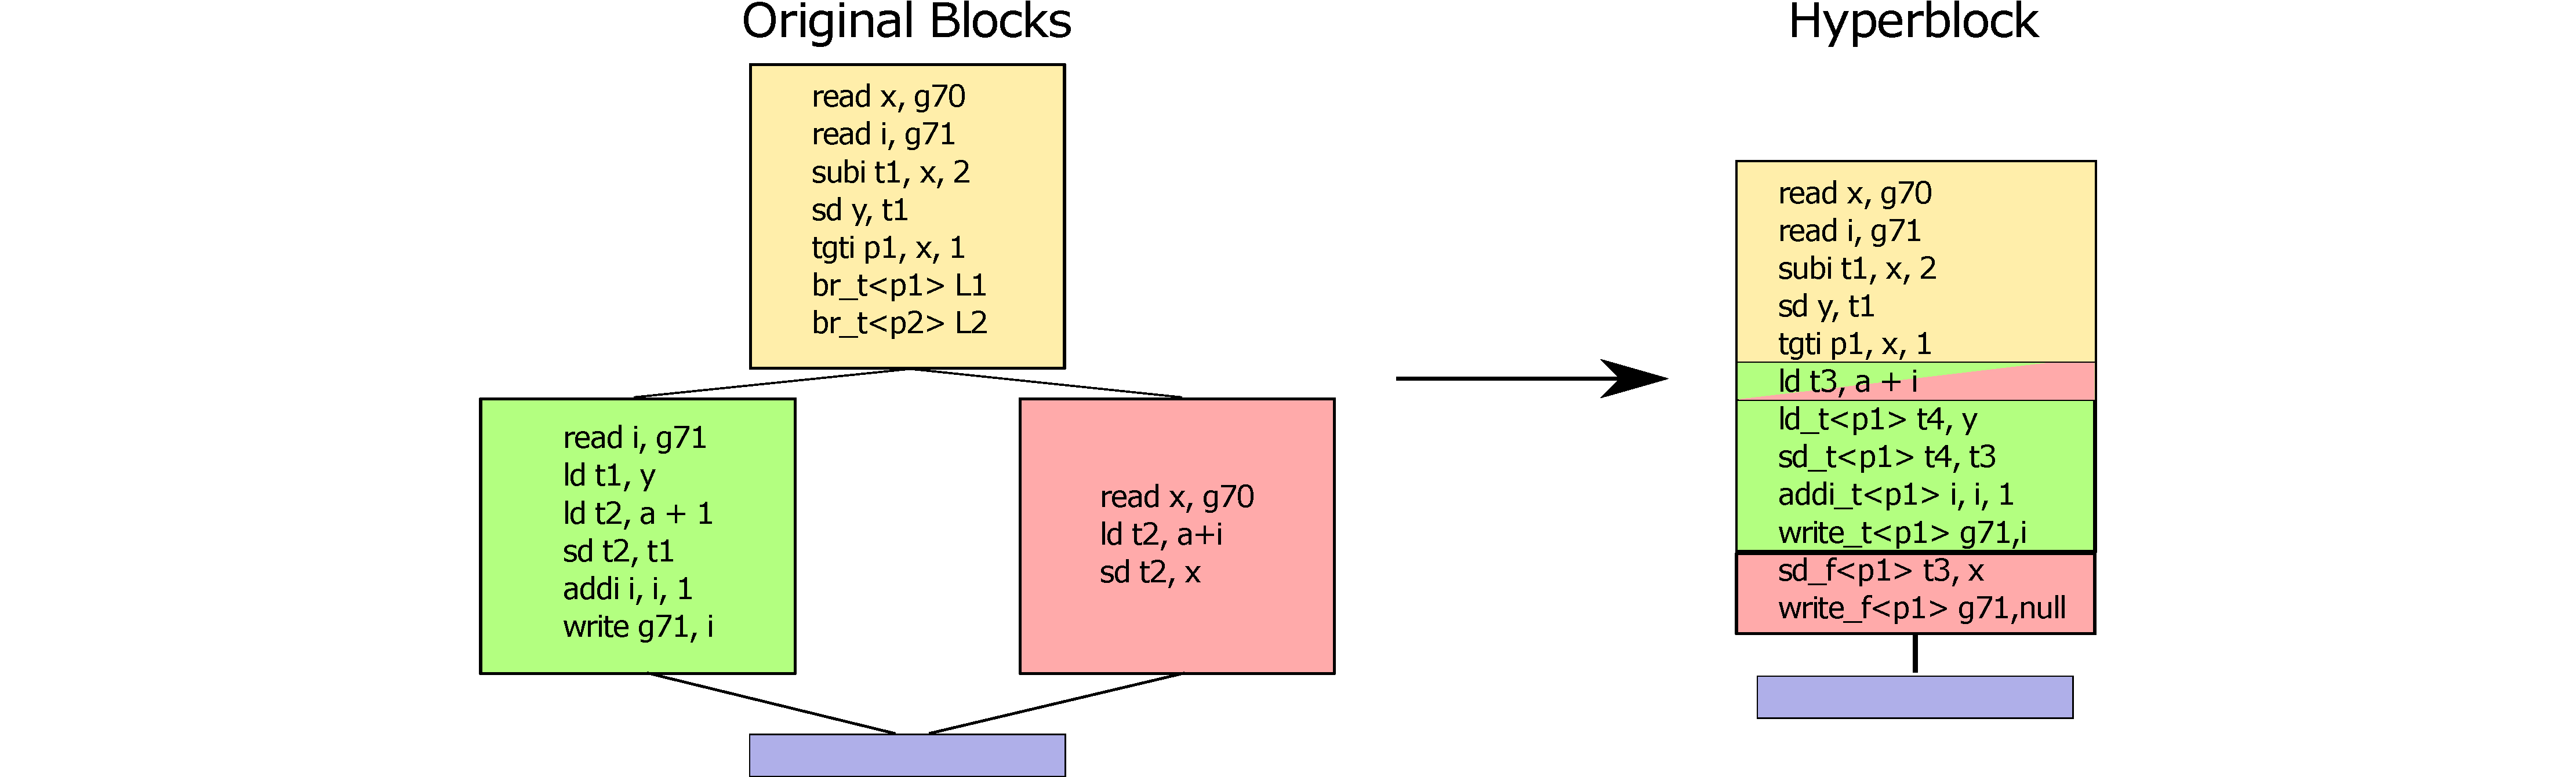
\includegraphics[width=1\textwidth]{background/graphics/hyperblock.pdf}
    \caption{High-level view of hyperblock formation. The three top blocks can be fused into a single block using instruction predication.}
    \label{fig:EdgeHB}
\end{figure}
To increase the size of EDGE blocks, multiple blocks can be combined together to form one large block called a hyperblock.
This is achieved through the use of instruction predication~\cite{smith2006edge}.
For example, the \textit{if/else} statement in the C code found in Figure~\ref{fig:EdgeHigh} normally generates two blocks, one for each statement.
However, using predication, the two blocks can be fused together and appended to the block that precedes the \textit{if/else}, reducing the number of blocks from 3 to 1.
Figure~\ref{fig:EdgeHB} shows the organisation of the new block, the box colour representing where the instructions originated.

As the compiler needs to declare stores and which registers are written to in the block header, extra instructions may need to be generated to ensure the block always executes the same amount of stores.
In the case of Figure~\ref{fig:EdgeHB}, the last instruction is generated to ensure that a write to the register \textit{g71} always happens regardless of the predicate.
This adds some complexity to hyperblock formation, as the size of the block may be artificially inflated if the merging blocks write to different registers or have a different number of stores.
Even so hyperblocks allow for increased instruction level parallelism (ILP) as  which in turn improves the performance of the application being executed~\cite{smith2006edge}.

Overall, the EDGE ISA enables the architecture to dispatch blocks speculatively, with low overhead~\cite{putnam2010e2,kim2007tflex}, therefore, increasing exploitation of ILP.

 \begin{figure}[t]
 \center
 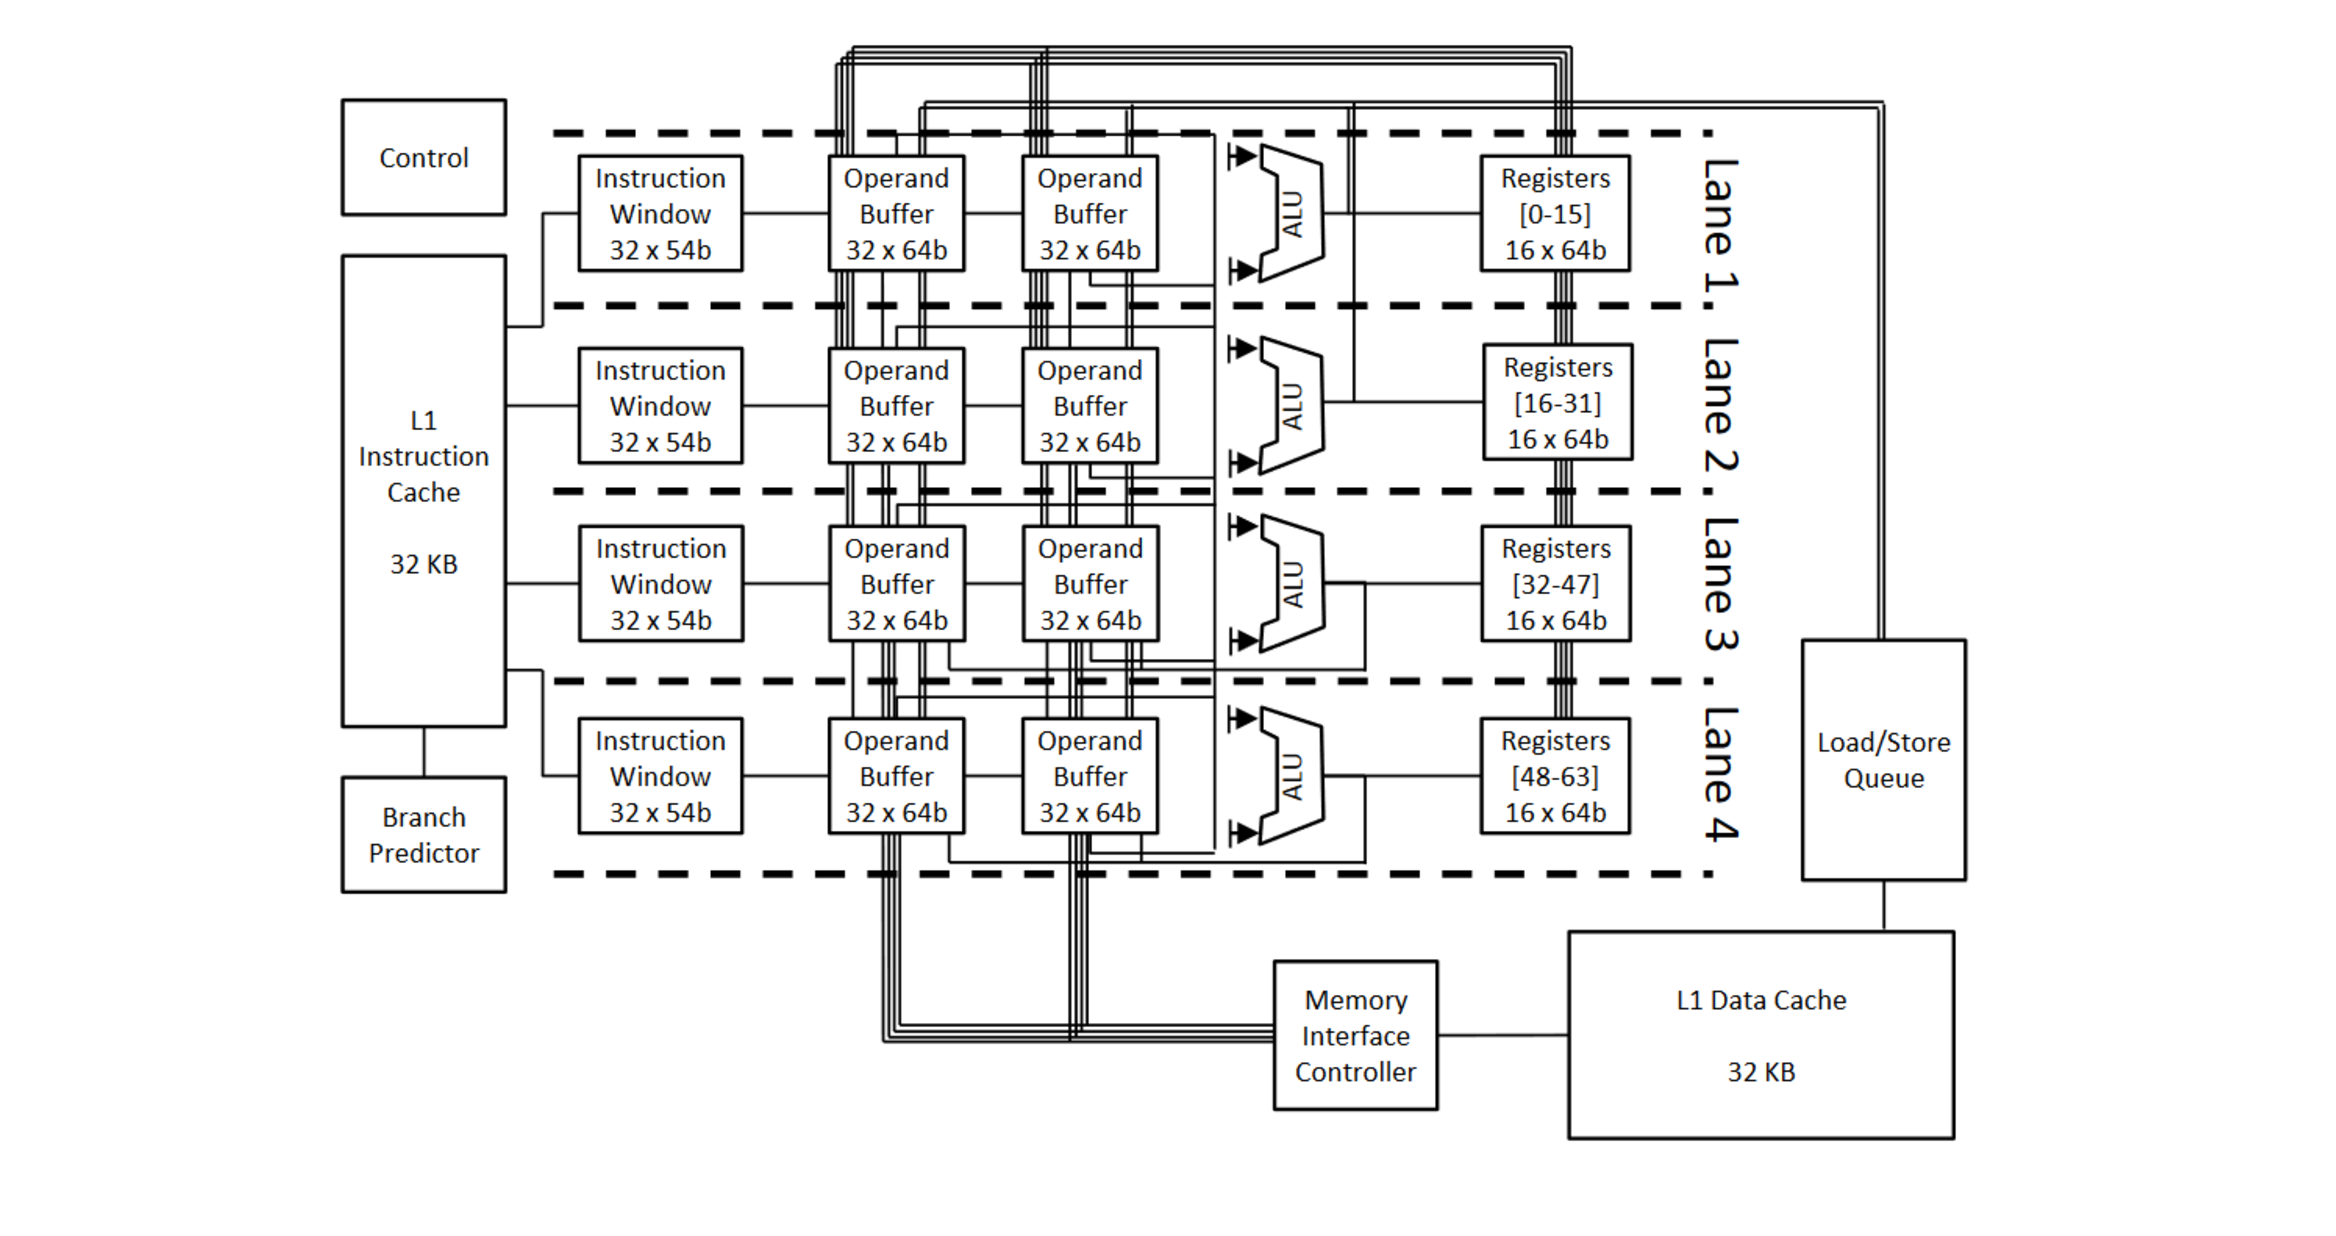
\includegraphics[width=1\textwidth]{background/graphics/edge_lanes.pdf}
 \caption{Example of a 4 lane core on an EDGE processor taken from~\cite{putnam2010e2}. The instruction window is split into 4 lanes, each can fetch a block of up to 32 instructions.}\label{fig:e2segment}
\vspace{-0.5em}
 \end{figure}

\subsection{EDGE Processor features}~\label{sec:edge_arch}

This section covers two important features of an implementation of EDGE processor called E2~\cite{putnam2010e2}.
The two features are the segmentation of the instruction window, and the core-composition mechanism used throughout this thesis.

\subsubsection{Core Lanes} 

According to Smith et al. in ~\cite{smith2006edge}, the sizes of blocks generated by the compiler for a set of applications from SPEC2000~\cite{spec2000} and EEMBC~\cite{eembc} range from 5 instructions to 50 instructions and on average are 20.6 instructions long.
If an EDGE processor is designed to fetch large blocks, which can be up to 128 instructions long, then the compiler is currently not able to generate large enough blocks.
To maximise core-utilisation, an EDGE processor instruction window can be segmented into lanes.
This allows the core to fetch more than a single block at a time.

Figure~\ref{fig:e2segment} shows a schemata for a four-lane EDGE core.
Given that a block in EDGE can be up to 128 instructions long, each lane is allowed to fetch a block of up to 32 instructions.
Fetching blocks larger than 32 instructions results in more than one lane being occupied by a single block.
Depending on the architectural setup, lanes may either share ALUs or they may have private ALUs.
As the instruction window is segmented, a core can continue fetching blocks until all its lanes are filled, allowing the processor to have multiple blocks in flight per core.
A segmented instruction window therefore allows EDGE cores to be more flexible to block size variability.

\subsubsection{Core Composition Functionality}\label{chp:Background:sec:EDGE}

Core Composition is achieved by fusing a set of \textit{physical} cores to create a larger \textit{logical} cores.
This does not modify the physical structure of the processor, instead it provides a unified view of a group of physical cores to the software.
In the processor used throughout the thesis, the micro-architecture is distributed: register files, Load Store Queues (LSQs), L1 caches and ALUs all look like nodes on a network.
This means that when cores are composed together, this is similar to adding an extra node to the network.
Core composition is a dynamic modification and may occur during the execution of a program to better fit the workload.
Unlike traditional CMPs, composed cores operate on the same thread and extract Instruction Level Parallelism (ILP) rather than Thread Level Parallelism (TLP)~\cite{micolet2016dmpstream,pricopi2012bahurupi}.

\begin{figure}
 \center
 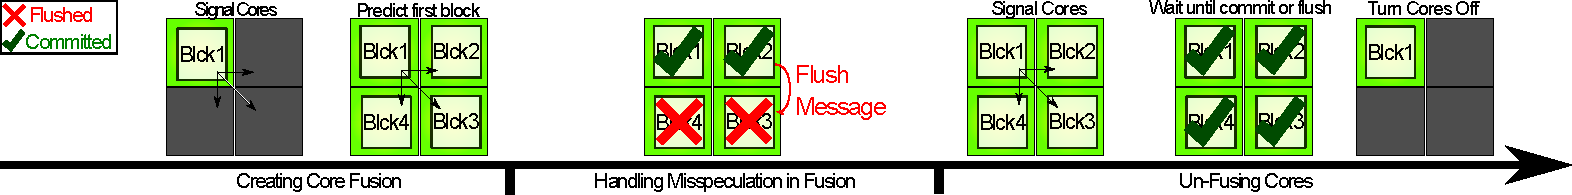
\includegraphics[width=1\textwidth]{cases-paper/graphics/background/proc_test.pdf}
 \caption{Core Composition Mechanisms for our EDGE-based architecture.}\label{fig:dmp}
 \end{figure}
 
Figure~\ref{fig:dmp} shows the different stages and mechanisms of core composition for a four core EDGE system.
When creating a new composition a master core informs all other cores about the fusion and sends the predicted next block address to an available fused core.
When a new thread is started on a fused core the OS and runtime write the new core mapping to a system register.
The hardware then flushes these cores if they are not idle and sets the PC of the first block of that thread on one core in the composition and starts executing.
When a core mispredicts a branch in a composition, it informs the other cores which flush any younger blocks.
When un-fusing, the master core informs the other cores, which then commit or flush their blocks and power down while the master core continues to fetch and execute blocks from the thread.
The extra hardware required to support dynamic reconfiguration is very minimal~\cite{kim2007tflex} since most of the machinery already in place can be reused such as the cache coherence protocol when fusing and un-fusing the cores.

When a composition fetches multiple blocks, it executes them out of order.
However instructions that modify memory or registers pass through the LSQ and register-file respectively and are executed in order to ensure memory and register value consistency.
In case of a memory violation caused by undetected dependencies a flush of all blocks younger than the violator, including the violating block, is performed.

\section{Value Prediction}~\label{sec:valpred}
%This will go in the background most likely
In Out of Order (OoO) superscalar processors, instructions can be executed out of order to improve ILP.
However, some instructions may depend on results from previous instructions, or memory system responses, such as an L1 cache response.
These data dependencies reduce the potential ILP, which in turn limits performance.

Value Prediction aims to provide a hardware solution to reducing latencies caused by memory dependencies in OoO superscalar processors~\cite{gabbayVPOrig} by predicting the values produced by instructions.
Instructions can be speculatively executed with predicted values as they wait for the real values to become available.
This is similar to branch prediction, where instructions from a predicted branch path are executed before the branch is resolved.
As long as the accuracy of the prediction is high, then executing the data-dependent instructions with speculative data increases ILP.

Until recently the benefits of using value prediction has been overshadowed by the potential power consumption and design complexity required to implement them \cite{peraisVTAGE2014}.
However, recent work by Perais et al.~\cite{peraisVTAGE2014,peraisBeBop2015} shows that by adopting the prediction and update scheme of the ITTAGE branch predictor~\cite{SeznecITTAGE}, and grouping predictions into blocks, value predictors be efficiently implemented.

\paragraph*{Type of predictors}
There exist two categories of value predictors \textit{Context} predictors and \textit{Computational} predictors.
In a \textit{Context} predictor, the predicted value of an instruction is based on capturing the history of values of the instruction.
This means that in a \textit{Context} predictor, a single instruction can occupy multiple entries of the predictor as each new value must be recorded.
The predicted value will then depend on the current context, which can either be captured by dataflow information or branch history~\cite{peraisVTAGE2014}.
This makes \textit{Context} predictors less efficient for predicting values that are incremented at a constant rate, as each increment occupies a new entry~\cite{peraisBeBop2015}.

On the other hand \textit{Computational} based predictors make a prediction by computing the value.
This can be achieved by detecting the delta between two commits of a value for an instruction, also known as the \textit{stride}.
Instead of storing each observed value for an instruction, a \textit{Computational} predictor stores the \textit{stride}, and the last committed value of an instruction.
When a prediction is requested, the \textit{Computational} predictor fetches the last committed value and the stride and adds them together to produce the prediction.
This allows \textit{Computational} to potentially reduce the size of the predictor as it only requires a single copy of the value to make a prediction. 


\subsection{The Differential Value Tagged Geometric length Predictor}~\label{chp:bck:vtage}
\vspace{-1em}
\begin{figure}[t]
    \centering
    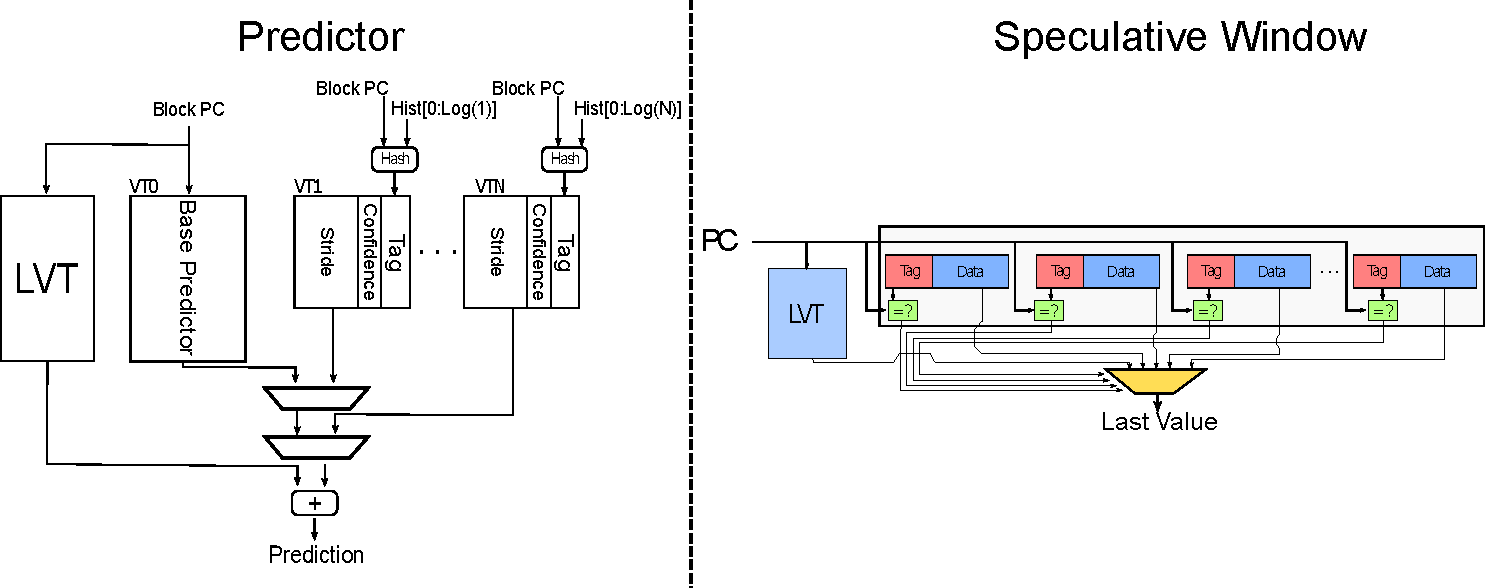
\includegraphics[width=1\textwidth]{background/graphics/valuepred.pdf}

    \caption{VTAGE stride-based value predictor and Speculative Window.}
    \label{fig:stride_over}
	\vspace{-1em}
\end{figure}
\subsubsection{Predictor mechanisms}
The D-VTAGE predictor~\cite{peraisBeBop2015} is a Computational value predictor that operates on blocks of instructions to minimize network pressure and increase the prediction output per cycle.
To simplify the explanation of the predictor in this chapter, the size of the block is set to 1 instruction.
The predictor is organised in two parts, a Last Value Table (LVT) that contains the last committed values for a given set of instructions, and the second part is a set of value tables (VT) which contain strides.
The left hand side of Figure~\ref{fig:stride_over} shows an overview of the predictor with N stride tables.
The largest stride table is a tagless base predictor, whereas VT1 to VTN are tagged by hashing the Program Counter of the instruction with varying amounts of the branch history.

A predicted value does not have to be used immediately, as the instruction can be dispatched normally.
This means that the value predictor can be trained before a prediction is used.
Depending on the configuration of the predictor, a prediction is only used when the confidence counter is set to a specific value.
This allows value predictors to be very accurate~\cite{peraisVTAGE2014}, though it sacrifices coverage.

\paragraph*{Making a prediction}
All the tables of the value predictor are accessed in parallel using the Program Counter hashed with different amounts of the branch history.
The base predictor is directly indexed, whereas the tables VT1 to VTN are tagged.
The prediction used will come from the table that has the longest branch history.
If the confidence counter of the entry is equal to the firing value then the prediction is used, it not then the prediction is kept alive until the instruction is committed to validate it.

\paragraph*{Updating the predictor}
Predictions are validated at the commit phase of the instruction to simplify the hardware~\cite{peraisVTAGE2014}.
On a correct prediction, the entry that generated the prediction has its confidence counter incremented by one.
If the predictor mispredicts, the entry's confidence counter is reset to 0 and the entry is propagated to tables that use longer branch histories.
The prediction and update schemes are directly inherited from the Tagged Geometric (TAGE) branch predictor~\cite{SeznecITTAGE}.

\subsubsection{Speculative Window}
Another consideration is that multiple blocks of the same PC may be speculatively executing at the same time, which could cause data mis-predictions if the predictor is not updated.
As predictions are updated at commit time, this requires current live predictions to be in a speculative window so that new predictions may use the last predicted data and stride.
The right hand side of figure~\ref{fig:stride_over} demonstrates how the speculative window works. 
Instead of directly querying the value predictor, the last value table and speculative window are searched in parallel for a matching tag which in this case is the Program Counter (PC) of the block.
If there is a live prediction, then the data from that prediction is used instead of the predictor.


%Also check this~\ref{sheikLVP2017}

\section{Streaming Programming Languages}~\label{sec:bg:stream}

% % This section should explain what steaming programming is (remove all the details about each language)
% General purpose programming languages often propose very little support for programs that handle with a continuous flow of data.
% This results in having to design a set of complicated for loops to manage the streams of data.
% Having to deal with different rates of incoming and outcoming data also increases the complexity of writing these applications using a standard language.

Streaming programming languages are a branch of dataflow programming that focus on applications that deal with a constant stream of data.
These applications, such as audio or video decoding can be commonly found in mobile devices.
Unlike conventional programming languages such as C++, these languages abstract the concept of incoming and outgoing data to permit the programmer to focus on how the data should be treated.
Programs are described as directed graphs where nodes are functions and their edges represent their input and output streams. 
These languages offer primitives to describe such a graph~\cite{theis2002streamit} which expose parallelisable and serial sections of the application directly to the compiler. 
Rates of incoming and out-coming data can also be defined to facilitate load balancing optimisations~\cite{chen2005rawstream}.

Features of streaming programming languages make them an ideal language for targeting multicore processors.
The explicit data communication between the different tasks in the program, the ability to estimate the amount of work performed in each task and information about data rates between tasks allows the compiler to easily generate a multi-threaded application that can run on a dynamic multicore processor.
However, the main challenge consists of deciding how to map the different tasks onto threads and how to allocate the right amount of resources to maximize performance.


\begin{figure}[t]
    \centering
    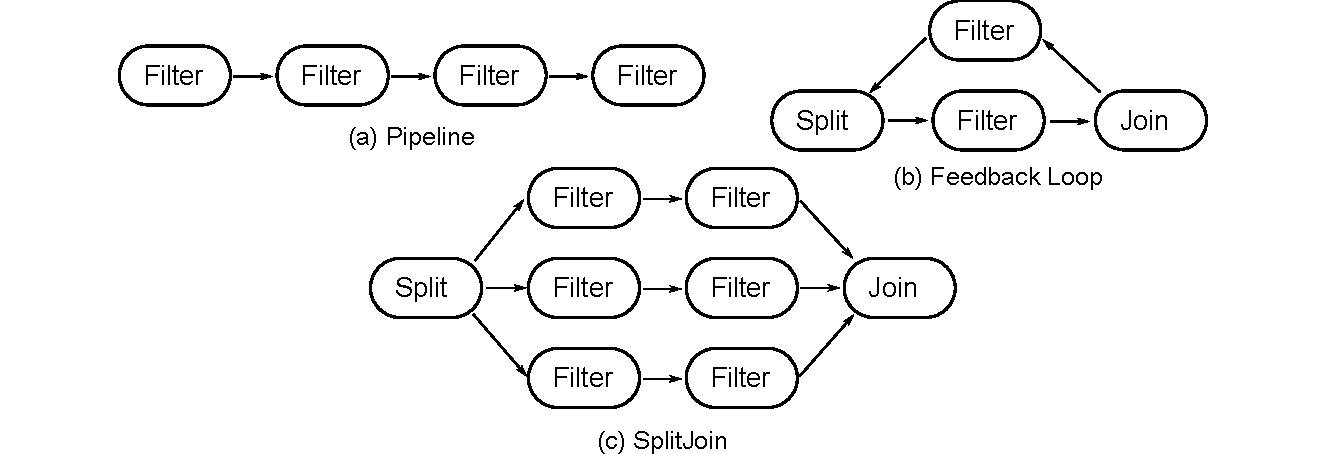
\includegraphics[width=1\textwidth]{streamit-paper/graphics/streamit_types.pdf}
    \caption{Visual representation of the three different StreamIt structures.}
    \label{fig:streamittypes}
\end{figure}

\subsection{StreamIt Programming Language}
StreamIt~\cite{theis2002streamit} is a high-level synchronous dataflow streaming programming language that defines programs as directed graphs.
StreamIt offers an elegant way of describing streaming applications, abstracting away how infinite data streams are managed to allow the programmer to solely focus on how the data must be treated.
A StreamIt program is composed of functions - called \textit{Filters} - which operate on streams of data.
Filters declare a certain amount of data which is to be consumed and produced per schedule.
Filters can be connected via \textit{Pipelines}, \textit{SplitJoins} or \textit{Feedback Loops} to create the streaming application.

Figure~\ref{fig:streamittypes} displays the different methods of connections in detail.
Pipelines (Figure~\ref{fig:streamittypes}(a)) represent a sequence of connecting filters operating on the same stream, each filter in the stream will operate on the output of the previous filter.
In a SplitJoin (Figure~\ref{fig:streamittypes}(c)), data from the stream is passed through a split filter and is either duplicated and passed on in parallel to the filters or distributed amongst the filters in a round-robin fashion.
The output of all the filters in a SplitJoin are then concatenated in a round-robin fashion through a joiner filter.
Finally a Feedback Loop (Figure~\ref{fig:streamittypes}(b)) provides a way for filters to operate on their outputs.
The resulting program written in StreamIt represents a graph where the nodes are filters and their edges represent the incoming and outgoing data streams.

\section{Machine-learning techniques and evaluation}~\label{sec:ml}
This section covers the different machine learning techniques and evaluation model used throughout the thesis.
The three techniques discussed are: linear regression, k-Means Clustering and k-Nearest Neighbours, whilst the evaluation technique is "leave-one out" cross validation.

\subsection{Linear Regression}~\label{sec:lr}

\begin{figure}[t]
    \centering
    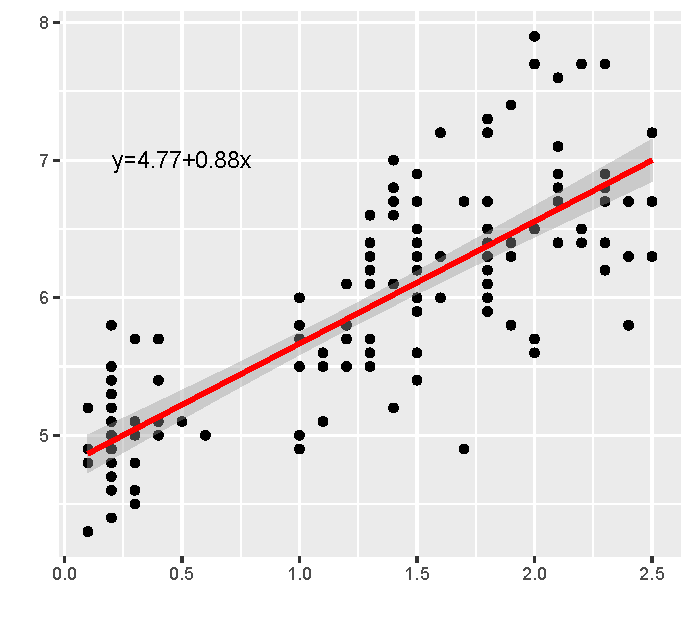
\includegraphics[width=0.45\textwidth]{background/graphics/lin_reg_ex.pdf}
    \caption{Example of linear regression. The inputs are represented by the circles, and the generated linear regression is represented by the red line.}
    \label{fig:linregex}
\end{figure}
Linear regression has previously been used to detect when to reconfigure hardware~\cite{tavanaElastic}.
Knowing when to reconfigure the processor necessitates fast decision making to minimize the overall cost of reconfiguration.
Machine learning models therefore need to be lightweight to ensure that the computations required to operate the model are as low as possible.
In these situations, a popular model is Linear Regression as it has a fairly low computational footprint~\cite{tavanaElastic}.

Linear Regression assumes a linear relationship between a set of inputs and the predicted output and generates a model in the form of:

\begin{equation}
y = \beta_0 + \beta_1X_1 + \beta_2X_2 + ... + \beta_nX_n
\end{equation}

where y is the predicted output, $X_{1..n}$ are the inputs and $\beta_{0.n}$ are weighted regression coefficients.
When training a linear regression, it generates the $\beta$ weights as to minimize the square-error between the training inputs and predicted outputs.
Once a model has been generated from input data, it can be implemented as a set of sums in hardware, making it an efficient way of making predictions.
Figure~\ref{fig:linregex} shows an example of a linear regression on a small dataset.
The linear regression takes the form of $y=4.77 + 0.88 \times x$ and is represented by the red line.

\subsection{k-Means Clustering}~\label{sec:kMeans}

\begin{figure}[t]
    \centering
    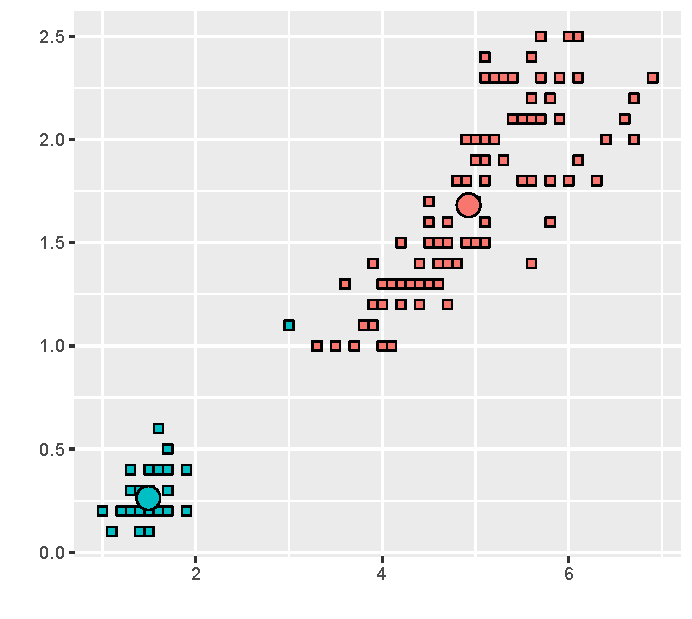
\includegraphics[width=0.45\textwidth]{background/graphics/smallest_clust_example.pdf}
    \caption{Small example of k-Means clustering with two clusters. The squares represent datapoints whilst the circles represent the centroids of the clusters.}
    \label{fig:kmeanex}
\end{figure}

k-Means is a clustering technique that groups \textit{n} observations into \textit{k} clusters such that $k < n$.
The original algorithm presented by Lloyd in ~\cite{kMeans} first randomly places \textit{k} centroids \textit{c} at random locations in the space.
Then, each point \textit{$x_{i}$} in the space of \textit{n} observations is assigned to a cluster who's centroid \textit{$c_{j}$} is closest to it.
Once each point has been assigned to a cluster, each centroid is recomputed by re-centering itself around the datapoints in the cluster.
This is repeated until the centroids no longer move.
 
Figure~\ref{fig:kmeanex} provides a visual example of a running k-Means on a toy dataset, with k set to two.
Each colour in the graph represents a cluster, the squares represent the n observations, whilst the circles represent the centroids.

\subsection{k Nearest Neighbors}~\label{sec:kNN}

\begin{figure}[t]
    \centering
    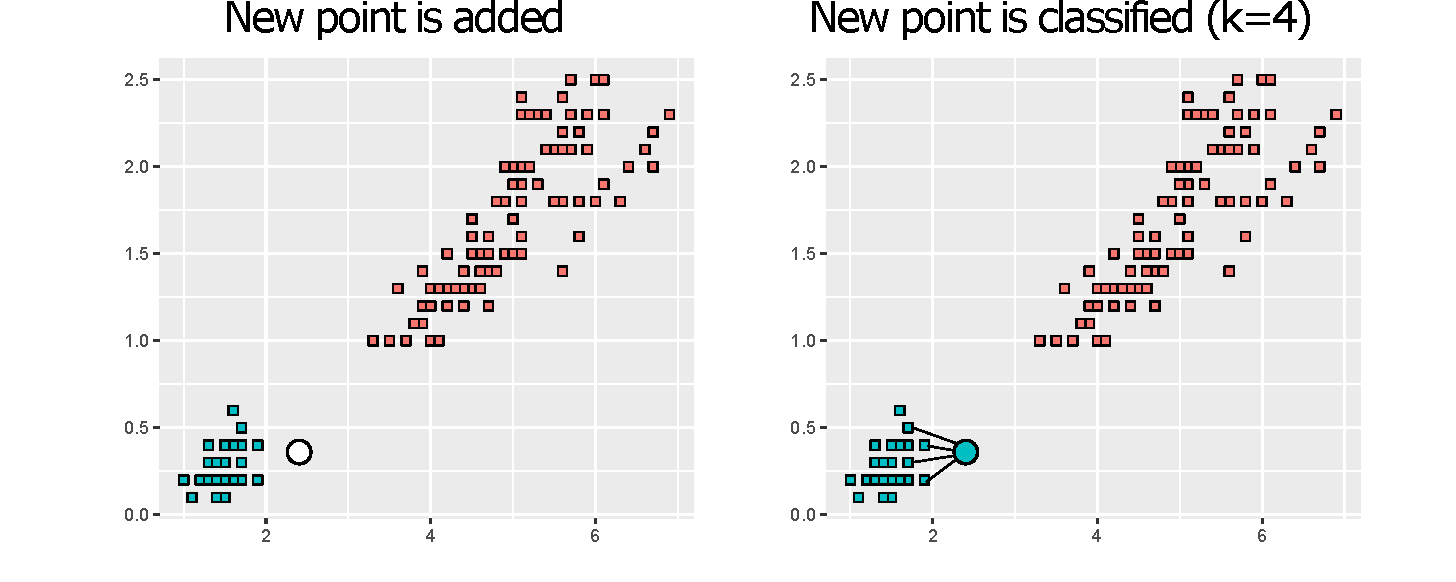
\includegraphics[width=1\textwidth]{background/graphics/knn1.pdf}
    \caption{Small example of k Nearest Neighbors classification on a toy dataset with two clusters and k = 4. The squares represent datapoints of the trained kNN dataset. The figure shows a new point (circle) being classified.}
    \label{fig:knn}
\end{figure}
k Nearest Neighbors (kNN) can be used for both regression and classification.
In both situations an output is generated by averaging the \textit{k} nearest neighbors to the input from the training data.
The average is often obtained by a weighted sum of the features of the k neighbors.
Figure~\ref{fig:knn} shows an example of a kNN classification on a new point.
The squares represent the trained kNN dataset, the colours represent the different classifications.
When a new point is added (as seen on the right hand graph), the four closest neighbors are found, and the new point is classified under the same category.

\subsection{Leave One Out Cross Validation}~\label{sec:valid}
The process of leave one out cross validation involves using the training dataset as the evaluation dataset.
Given a set of $n$ points in the training set, a new model is trained using $n-1$ of the points available.
The last unused datapoint is evaluated against this new model.
This procedure is repeated for every point in the dataset, and the results of the evaluation are averaged out to produce a final result.
This validation model works well when the number of testing and training data is small.
\newpage
\section{Early Stopping Criterion}~\label{sec:esc}

When exhaustive search of an optimisation space is not feasible, a subset of the space is explored.
The early stopping criterion (ESC)~\cite{vuduc2003AutomaticPerf} provides a method of determining when new points added in the subspace no longer provide new information, and thus the currently evaluated subspace is representative of the total space.
Given $N$ possible number of implementations, if $i$ is a single implementation and $x_i$ is its performance normalised between 0 and 1, then $S=\{x_1,...,x_N\}$ is the set of all performances for all possible implementations.
If $X$ is a random variable corresponding to a randomly selected performance from the set S then there is a cummulative distribution function (CDF) $F(x) = Pr[X \le x]$ which is equal to the number of items in S that are less than or equal to $x$ ($n(x)$) over all possible items $N$.
If, for a number of time steps, a performance from S is randomly chosen and not replaced, then at time step $t$ $M_t$ is maximum performance observed $max_{1\le i \le t} Xi$ up to time t.
ESC posits that, that if the probability that $M_t$ is within a distance of the maximum performance found in S then the space exploration can stop at time t.
Formally, ESC is:
\begin{equation}
Pr[M_t \le 1 - \epsilon ] < \alpha
\end{equation}

Where $\epsilon$ is the proximity to the best performance in $S$ and $\alpha$ is the uncertainty factor.
For example, if the user wants to stop the search when $M_t$ is within 5\% of the best, with an uncertainty factor of 10\% they would set $\epsilon$ to 0,05 and $\alpha$ to 0,1.

As ESC is used when the exhaustive space has not been searched, the set of all performances $S$ is unknown.
Instead, ESC uses an approximation of the space, using the set of already observed performances rather than $S$.
The approximation is determined via this formula:
\begin{equation}
\hat{G}_t(x) = \frac{ \binom{\ceil*{N \times \hat{F}_t(x)}}{t}}{\binom{N}{t}}
\end{equation}

Where $\hat{F}_t(x)$ is the CDF for the random variable X given the set of observed performances at time $t$.
Finally, using the approximation, ESC can be defined as:

\begin{equation}
\hat{G}_t(1-\epsilon) < \alpha
\end{equation}
